\section{DPDK(Data Plane Development Kit)}
\label{sec:DPDK}
本章では,DPDKによるパケットI/Oとその実行モデルについて述べる.また,カーネルによるパケットI/OとDPDKによるパケットI/Oの比較やDPDKによるパケットI/Oの問題点についても述べる.

\subsection{DPDKによるパケットI/O}
DPDK \cite{DPDK} とは2010年にIntelによって作られたパケット処理を高速化するためのライブラリである.

DPDKは特定のCPUコアを占有することによって,NICを常時ポーリングで監視する.そのため,DPDKによるパケットI/O(図\ref{fig:DPDKPacketIO})では,一定時間に受信するパケットの量が増えると,コンテキストスイッチが増加して,割り込み以外の処理ができなくなってしまう問題は発生しない.

また,DPDKによるパケットI/Oでは,NICは受信したパケットをユーザ空間からアクセス可能な主記憶領域に書き込む.そのため,受信したパケットをカーネル空間からユーザ空間にコピーしなくても,ユーザ空間のアプリケーションがパケットにアクセスすることができる.

\begin{figure}[htb]
  \centering
  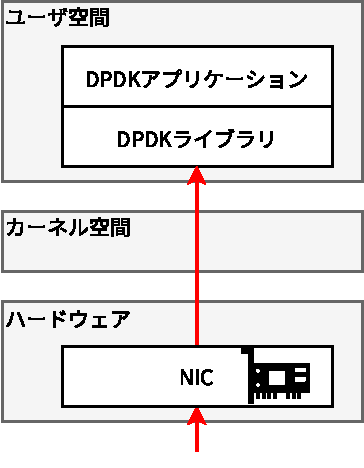
\includegraphics[width=0.5\columnwidth]{pictures/DPDKPacketIO.pdf}
  \caption{DPDKによるパケットI/O}
  \label{fig:DPDKPacketIO}
\end{figure}

\subsection{DPDKの実行モデル}
DPDKの実行モデルにはRun-to-CompletionモデルとPipelineモデルの二つがある.Run-to-Completionモデルは受信処理,パケット処理,送信処理を一つの論理コアで行うモデルである(図\ref{fig:RunToCompletion}).パケット処理が重たいと受信処理にCPUリソースが割当たらなくなり,パケットロスが生じてしまうため,パケット処理ではパケットヘッダの書き換えといった軽い処理が一般的には行われる.Pipelineモデルは受信処理,パケット処理,送信処理をそれぞれ別の論理コアで行うモデルである(図\ref{fig:Pipeline}).受信処理を行う論理コアとパケット処理を行う論理コアが別であるため,パケット処理が重たくてもパケットロスが生じることはない.しかし,CPUのL1キャッシュを有効活用できない.また,それぞれの処理が論理コアを占有するため,分散計算環境においてはコアの使用効率が悪い.

\begin{figure}[htb]
  \centering
  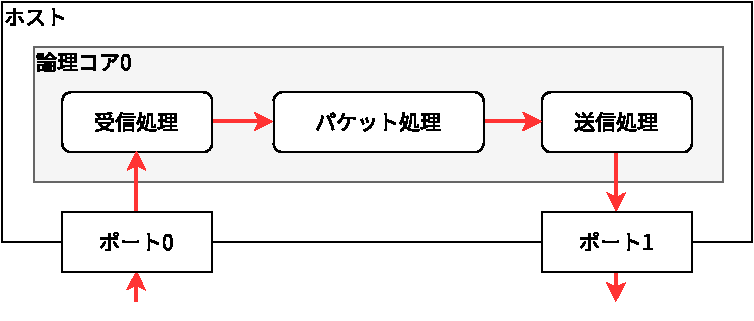
\includegraphics[width=\columnwidth]{pictures/RunToCompletion.pdf}
  \caption{Run-to-Completionモデル}
  \label{fig:RunToCompletion}
\end{figure}

\begin{figure}[htb]
  \centering
  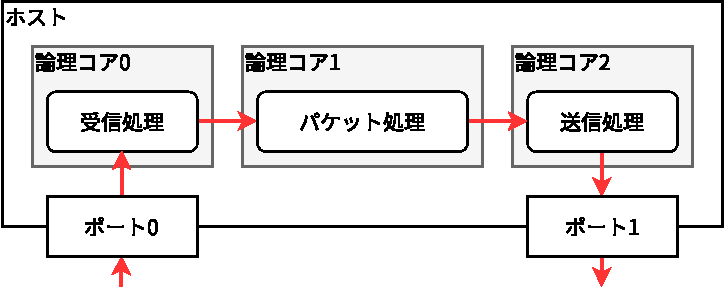
\includegraphics[width=\columnwidth]{pictures/Pipeline.pdf}
  \caption{Pipelineモデル}
  \label{fig:Pipeline}
\end{figure}

\subsection{パケットI/Oの比較}
文献 \cite{XDP} で調査された,カーネルによるパケットI/OとDPDKによるパケットI/Oの通信スループットを図\ref{fig:PacketIOComparison}に示す.このグラフの横軸は使用したCPUコアの数,縦軸は受信したパケットをすべてドロップしたときのスループットを表している.また,緑の折れ線はDPDKによるパケットI/O,ピンクの折れ線はカーネルによるパケットI/Oを表している.グラフより,DPDKのスループットはカーネルのスループットに比べて最大8倍程度高いことがわかる.

\begin{figure}[htb]
  \centering
  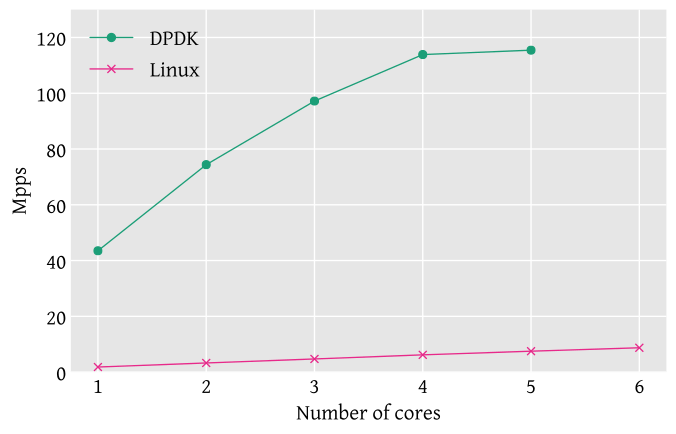
\includegraphics[width=\columnwidth]{pictures/PacketIOComparison.png}
  \caption{パケットI/Oの比較}
  \label{fig:PacketIOComparison}
\end{figure}

\subsection{DPDKによるパケットI/Oの問題}
DPDKは特定のCPUコアを専有することによって,NICを常時ポーリングで監視するため,通信スループットが低いときでもCPUリソースを無駄に使ってしまう.文献 \cite{XDP} で調査された,カーネルによるパケットI/OとDPDKによるパケットI/OのCPU使用率を図\ref{fig:DPDKProblem}に示す.このグラフの横軸は通信スループット,縦軸はCPU使用率を表している.また,緑の折れ線はDPDKによるパケットI/O,青の折れ線はカーネルによるパケットI/Oを表している.グラフから,カーネルによるパケットI/OのCPU使用率は通信スループットが高くなるにしたがって徐々に増えていくことがわかる.それに対して,DPDKによるパケットI/OのCPU使用率は通信スループットにかかわらず常に100\%であることがわかる.

\begin{figure}[htb]
  \centering
  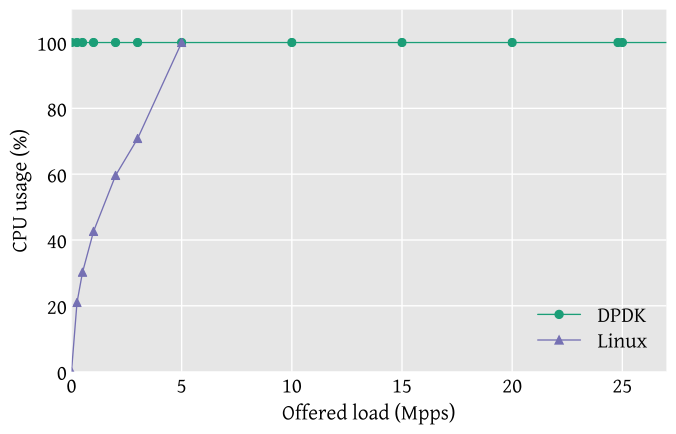
\includegraphics[width=\columnwidth]{pictures/DPDKProblem.png}
  \caption{DPDKによるパケットI/Oの問題}
  \label{fig:DPDKProblem}
\end{figure}
